\documentclass[border=10pt]{standalone}
\usepackage{verbatim}
\usepackage{amsmath, calc}

\usepackage{tikz}
\usetikzlibrary{shapes, shadows, arrows}
\usetikzlibrary{positioning}
\usepackage{xcolor}

\begin{document}
    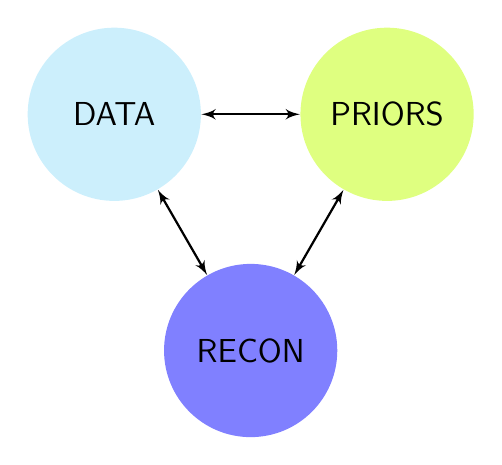
\begin{tikzpicture}\sffamily


        \begin{scope}[blend group = soft light]
            \node[fill=lime!50!white, circle, minimum size=2.2cm] (A) at  (30:2) {};
            \node[fill=cyan!20!white, circle, minimum size=2.2cm] (B) at  (150:2) {};
            \node[fill=blue!50!white, circle, minimum size=2.2cm] (C) at  (270:2) {};
        \end{scope}
        
        \node[inner sep=5pt]  at (30:2) {\large PRIORS};
        \node[inner sep=5pt]  at (150:2) {\large DATA};
        \node[inner sep=5pt]  at (270:2) {\large RECON};

        \draw[latex'-latex', thick, black] (A) to (B);
        \draw[latex'-latex', thick, black] (A) to (C);
        \draw[latex'-latex', thick, black] (B) to (C);
        
    \end{tikzpicture}
    
\end{document}